\begin{frame}
  \frametitle{Automation}
  \begin{figure}[htpb]
      \raggedleft
      
\includegraphics[width=2cm]{images/robot-icon.eps}
      \newline
      {\tiny Source: \cite{robot_icon}}
  \end{figure}

  Automating out repetive tasks saves more time for designing and developing features and bug fixes.
  \newline
  \newline
  Question: How do we implement automation?
  \pause
  \newline
  \newline
  Answer: Using an {\it automation framework}.

\end{frame}

\begin{frame}[t]
    \frametitle{Automation Framework}
    \begin{figure}[htpb]
        \begin{subfigure}
            \centering
            
\includegraphics[width=3cm]{images/circleci-logo.png}
        \end{subfigure}
        \hspace{1cm}
        \begin{subfigure}
            \centering
            
\includegraphics[width=3cm]{images/github-actions-logo.png}
        \end{subfigure}
        \newline
        {\tiny Sources: \cite{circle_ci_logo}, \cite{github_actions_logo}}
    \end{figure}

    Automation frameworks are services execute user-created instruction sets called {\it workflows} when certain conditions, or {\it triggers}, are met.

    Automation frameworks can read files from the main host repository. This enables users to create workflows to do things like:
    \begin{itemize}
        \item automatically run a test suite whenever the code changes ({\it continuous integration})
        \item build and deploy online documentation
        \item manage repository metadata
    \end{itemize}
    
\end{frame}

\begin{frame}
    \frametitle{GitHub Actions}
    
    GitHub Actions is an automation framework integrated into every GitHub repository.

    \begin{figure}[htpb]
        \centering
        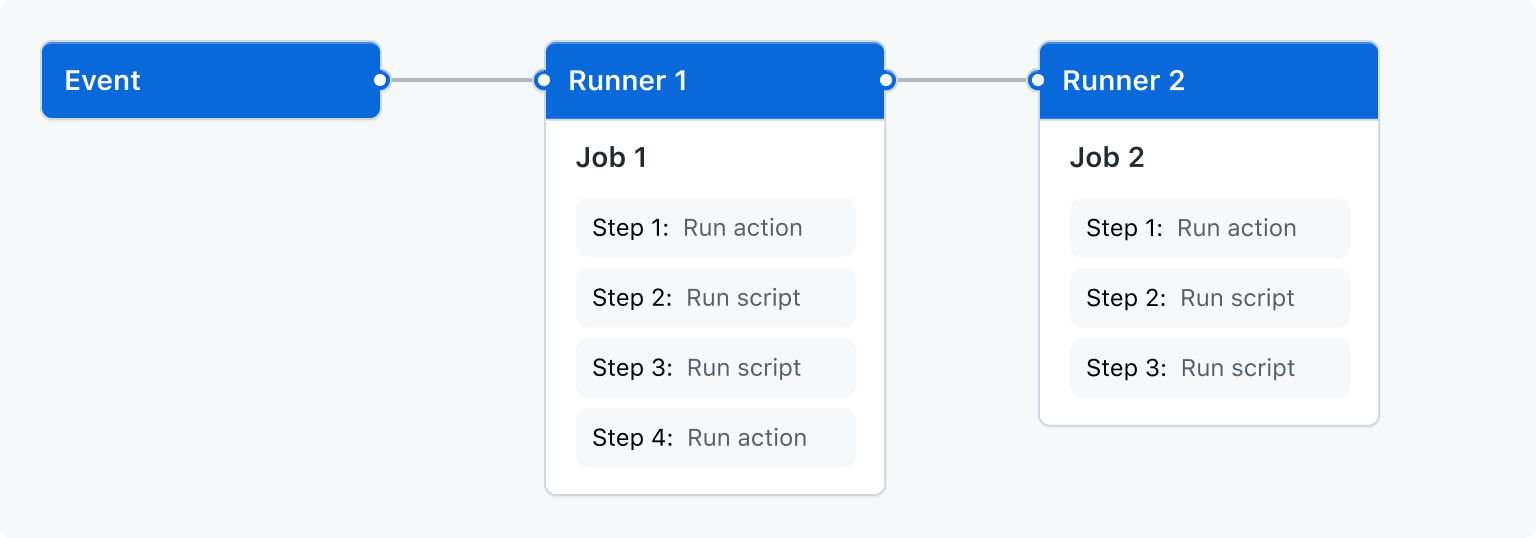
\includegraphics[width=10cm]{images/overview-actions-simple}
        {\tiny Source: \cite{github_actions_conceptual_example}}
    \end{figure}

    The basic workflow file structure is as follows:
    \begin{itemize}
        \item Workflow name
        \item Define workflow triggering events
        \item Define the workflow jobs and steps
    \end{itemize}

\end{frame}

\begin{frame}
    \frametitle{GitHub Actions Workflow Example}
    \framesubtitle{Populating SaltProc release notes}

    \begin{figure}[htpb]
        \centering
        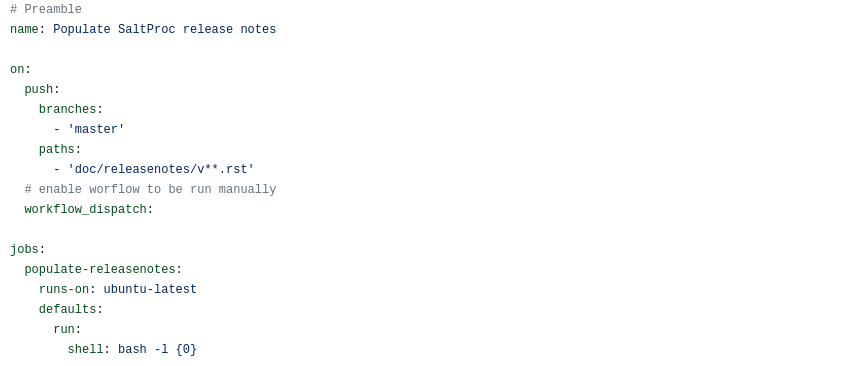
\includegraphics[width=10cm]{images/github_actions_workflow_ex1}
    \end{figure}

\end{frame}

\begin{frame}
    \frametitle{GitHub Actions Workflow Example}
    \framesubtitle{Populating SaltProc release notes}

    \begin{figure}[htpb]
        \centering
        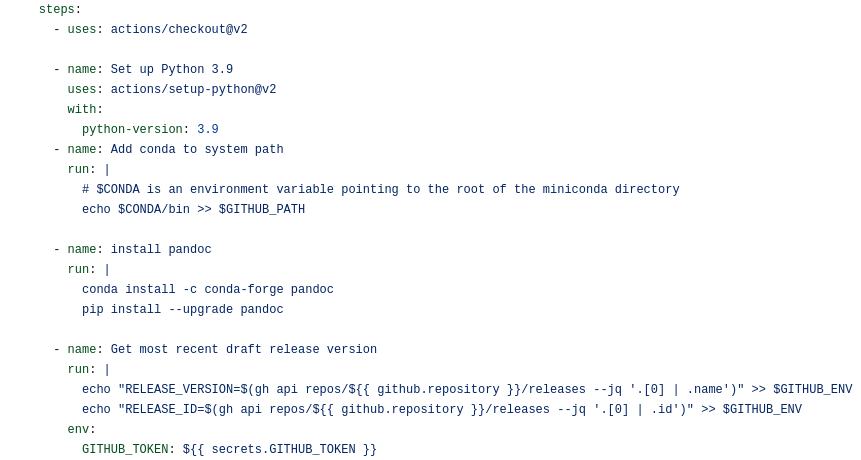
\includegraphics[width=10cm]{images/github_actions_workflow_ex2}
    \end{figure}
\end{frame}

\begin{frame}
    \frametitle{GitHub Actions Workflow Example}
    \framesubtitle{Populating SaltProc release notes}

    \begin{figure}[htpb]
        \centering
        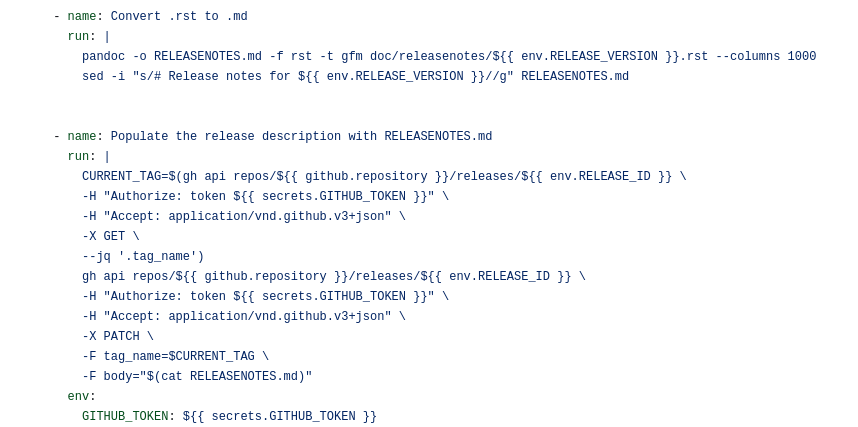
\includegraphics[width=10cm]{images/github_actions_workflow_ex3}
    \end{figure}
\end{frame}


